\section{Selection}

This analysis uses the full $3.0\invfb$ of data collected by the \lhcb
experiment~\Ref{Alves:2008zz} in the years 2011 and 2012 at 7 and $8\tev$ respectively.
Since the properties of the \db are unknown, a variety of simulated samples of the decay \btokstrdb,
where \dbtomumu, were generated with a range of \mass{\db} and $\tau_\db$, a summary of these are
shown in \Table{tab:db:samples}.
Also used in this analysis, are simulated events of the decays \btokstrmumu and \btojpsikstr.

\begin{table}
  \caption[Samples of simulated \btokstrdb generated for the analysis]{
    Samples of simulated \btokstrdb generated with given mass and lifetime.
    A total of 1.5 million events are generated for each sample, but only 1.5 thousand for the
    samples with a \mass{\db} of 220 and $235\mev$.
  }
  \label{tab:db:samples}
  \begin{center}
    \begin{tabular}{rccccccccccc}\toprule
    %\begin{tabular*}{\textwidth}{r @{\extracolsep{\fill}} ccccccccccc}\toprule
      $\tau_\db$ (ps) & \multicolumn{10}{c}{\mass{\db} (MeV)} \\\midrule
      10 &&&&&&&&&2500 \\
      100 &214&220&235&250&500&800&1000&1500&2000&2500&4000 \\
      1000 &&&&250&&&&&2500 \\
      \bottomrule
    \end{tabular}
    %\end{tabular*}
  \end{center}
\end{table}

Reconstructed decays of \btokstrdb are required to fire the \lone triggers for muon, dimuon, or
hadronic candidates.
Subsequent trigger levels require that the decay has a topology consistent with a $B$-meson
decaying in to a multi-body final state which includes muons.
Only \TOS candidates are used in this analysis for two reasons: firstly, the ratio of trigger
efficiency for the \sm \btokstrmumu to that of (possibly displaced) \db mode enters
into the limits and, thus, must be precisely determined; and the use of \TIS events would
come with a substantial enhancement of the di-$b$-hadron backgrounds.
The few percent gain in signal efficiency obtained using \TIS is not worth the increase in these
backgrounds  di-$b$-hadron backgrounds.

Candidates for the decay \btokstrdb, where \dbtomumu are reconstructed allowing that the \db can
be displaced from the decay vertex of the \Bd.
Since the \db could be a long-lived particle, and travel beyond the acceptance of the \velo before
it decays, it is prudent to consider the use of \emph{downstream} tracks.
Track types are defined by which tracking subdetectors in which they are observed,
\Fig{fig:db:lldd} shows these various definitions.
For most \lhcb analyses, the only appropriate track to use are \emph{long} tracks, which have hets
in each tracking station; long tracks are used in the analyses described in \Chap{ch:hits} and
\Chap{ch:hhh}.
The problem with using downstream tracks is that they are not triggered efficiently in \hlttwo.
For example, a simulated \db with a mass of $250\mev$ and a lifetime of $100\ps$ has a
reconstruction and
stripping efficiency of \approx$0.9\pc$ if the muons are both long tracks, but the equivalent
number for downstream tracks is \approx$2.5\pc$; due to the boost of a light object from a decaying
\Bd.
However, the trigger efficiency for this sample is \approx$45\pc$ and $8\pc$ for long and
downstream candidates respectively.
There is therefore a factor two more long-track candidates for the $250\mev$ $100\ps$ sample; which
is a factor of a few hundred for more massive, or shorter lifetime, dark bosons.
For this reason, this analysis deals only with \db candidates formed from long-track muons.

\begin{figure}
  \begin{center}
    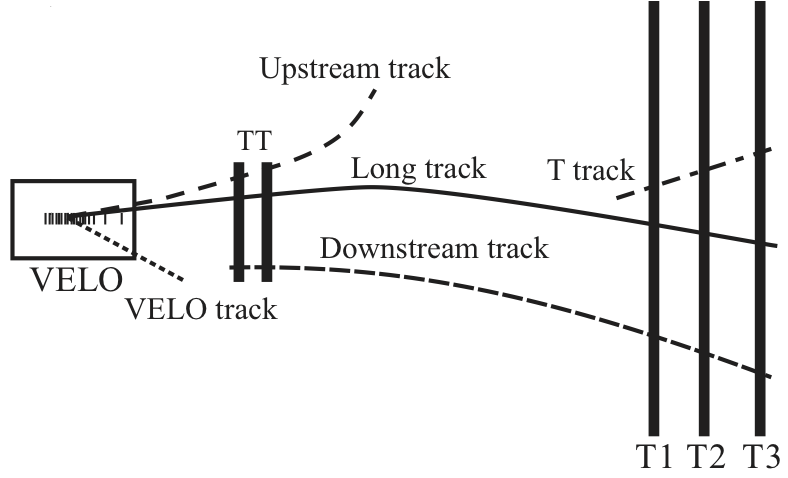
\includegraphics[width=0.48\textwidth]{track}
    \caption[Track definitions in the LHCb detector]{
      Schematic diagram of the \lhcb tracking system, showing the \velo, \ttracker, and tracking
      stations T1--3.
      Track types at \lhcb are defined by the regions through which they travel, as labelled in the
      diagram.
      Most tracks used in analyses are classified as long tracks, but for long-lived particles
      (such as the \KS) downstream tracks are often also used to increase statistics.
      This analysis focused on long tracks.
      %and tracking stations one, two, and three.
      %This analysis focuses on particles decaying into a pair of long tracks.
    }
    \label{fig:db:lldd}
  \end{center}
\end{figure}

%The selection
%Simulated samples are extremely important for this analysis,
%It is important to remove sources of background while leaving the invariant mass of the dimuon
%distribution smoothly varying, so that the assumption of local-linearity remains.
%In \Sec{sec:strategy} resonances are discussed, and those where $\Gamma<5\sigmam$ must be vetoed.
%For this analysis,


The offline selection criteria applied in the stripping are outlined in \Tab{tab:stripping}.
%The variable {\tt DOCA} is defined as the distance of closest approach between any two pairs of
%tracks in the candidate.
This table lists the variables {\tt ProbNNK} and {\tt ProbNNpi}, which are \MVA algorithms giving a
response $\in[0,1]$ quantifying how kaon or pion like a particle is, respectively.
The full decay chain \btokstrdb and \dbtomumu is reconstructed using a fit in which the \Bd mass is
constrained to its known value~\cite{PDG2014}.
All references to $m(\db)$, $m(\Kstar)$ or $\tau(\db)$ are to the values after this vertex fit
has been performed.

\begin{table}
  \caption[Stripping selection]
  {
    While the \Bd mass is constrained in the fit, the selection makes a cut on the unconstrained
    mass.
    %The variable {\tt DOCA} is defined as the distance of closest approach between any two pairs of
    %tracks in the candidate.
  }
  \label{tab:stripping}
  \begin{center}
    \begin{tabular}{llcrl}\toprule
      Candidate & \multicolumn{4}{c}{Cut} \\\midrule
      \Bp
      & $\chisqvtx/\ndf$          & $<$ & 25   \\
      & \chisqip                  & $<$ & 50   \\ % BPVIPCHI2
      & $\tau$                    & $>$ & 0.2 & ps  \\
      & $m$                       & $\in$ & $[4800, 5800]$  & MeV \\
      & \pt                       & $>$ & 1000    & MeV   \\
      & $\cos\theta_\mathrm{dir}$     & $>$ & 0 \\
      \littlerule
      \db
      & $\chisqvtx/\ndf$          & $<$ & 10   \\ % VCHI2DOF
      & $\chisqfd$                & $<$ & 25   \\
      & \pt                       & $>$ & 250  & MeV \\
      & DOCA                & $<$ & 0.2 & mm \\
      & DOCA \chisq         & $<$ & 25  &    \\
      \littlerule
      Tracks
      & $\chisqtrk/\ndf$          & $<$ & 3    \\
      & $\min(\chisqip)$                  & $>$ & 9    \\ % MIPCHI2DV
      & $\mathcal{P}_\mathrm{gh}$ & $<$ & 0.3  \\
      \littlerule
      $\Kp$, $\pip$
      & \pt                       & $>$ & 250  & MeV \\
      & $p$                       & $>$ & 2000 & MeV \\
      & \chisqip                  & $>$ & 9 \\
      \Kp
      & {\tt ProbNNK}             & $>$ & 0.1  \\
      \pip
      & {\tt ProbNNpi}            & $>$ & 0.2  \\
      \mup
      & \pt                       & $>$ & 100  & MeV \\
      & {\tt PIDmu}               & $>$ & -5   \\
      & \ismuon                   & & True \\
      \bottomrule
    \end{tabular}
  \end{center}
\end{table}


\subsection{Preselection}
After the stripping and triggering stages, a loose preselection is applied (see \Tab{tab:presel}).
The data sample is further purified using a multivariate algorithm, which is discussed in the
following subsection.
The preselection places cuts on topological quantities the combined efficiency of which is
\approx$90\%$ on all simulated samples.

Cuts are applied to the \Kstar and its daughters to remove candidates that are clearly
inconsistent with the decay  \decay{\Kstarz}{\kpi}.
Firstly, It is required that the invariant mass of the \decay{\Kstarz}{\kpi} candidate has a mass
within $100\mev$ of the known mass of the $K^*(892)^0$ meson, which has been measured to be
$(895.81\pm0.19)\mev$~\cite{PDG2014}.
\pid constraints are also applied to each \Kstar daughter: $\dllkpi(\Kp)>-5$, $\dllkpi(\pip)<25$;
and to ensure that the kaon candidate looks more like a kaon than the pion candidate a cut on the
difference in \glspl{DLL} is also applied: $\dllkpi(\Kp)-\dllkpi(\pip)>10$.

Another background from misidentified particles that is removed in the preseleciton is that of a
decaying \KS meson.
A \KS has a mass of $(497.61\pm0.02)\mev$~\cite{PDG2012}, a lifetime of
$(8.954\pm0.004)\e{-11}\sec$~\cite{PDG2012}, and decays
into two charged pions $(69.20 \pm0.05)\pc$ of the time.
If these two pions are misidentified as muons then there is significant peaking backround around
the \KS mass, becuase the mass of a muon and pion are similar.
To counter this, candidates are vetoed if the mass of $m_{\pi_\mu^+\pi_\mu^-}$ is within $25\mev$
of the known \KS mass.

Since the \db can be displaced from the \Db decay vertex, a potential background for the decay
\dbtomumu is from a \mumu pair directly from a \pv.
This is suppressed by requiring that the transverse flight distance (\FDT) of the \db vertex, with
respect to the \pv is greater than $0.1\mm$.

Similar to in \Sec{sec:hhh:sel}, the decay \btokstrdb suffers from backgrounds from
\decay{\Bd}{\jpsi\Kstarz} where a hadron is misidentified as a hadron and vice versa.
In this case the background can be suppressed by requiring that neither the \Kp nor the \pim
satisfy the \ismuon criteria.
The effect of this cut is shown in \Fig{fig:db:doublemisid}.
A summary of all preselection cuts are shown in \Tab{tab:db:presel}.

\begin{figure}
  \begin{center}
    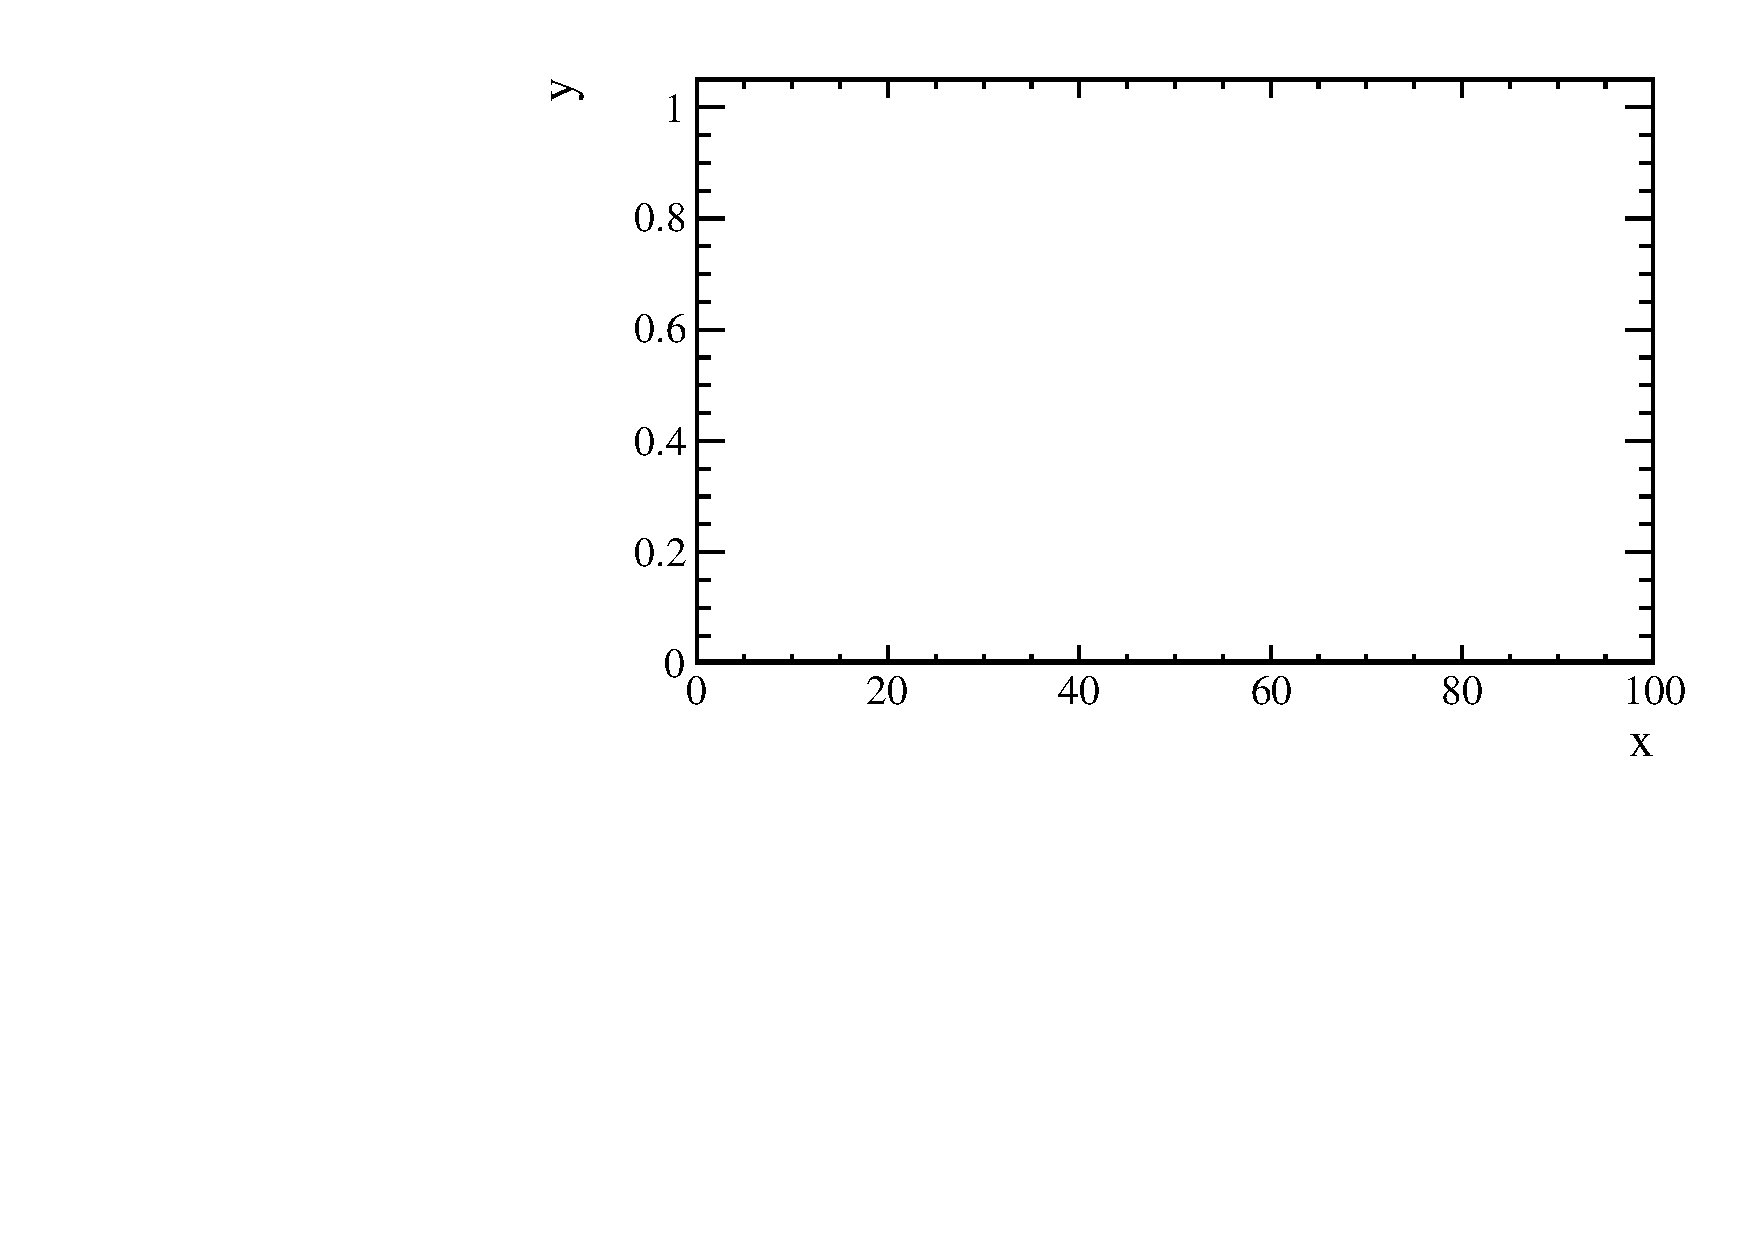
\includegraphics[width=0.48\textwidth]{blank}
    \caption{
      Duoble misid
    }
    \label{fig:db:doublemisid}
  \end{center}
\end{figure}

\begin{table}
  \caption[Preselection cuts] {
    Preselection cuts.
  }
  \label{tab:presel}
  \begin{center}
    \begin{tabular}{llcrl}\toprule
      Candidate & \multicolumn{3}{c}{Cut}\\
      \midrule
      \Bd
      & $\theta_\mathrm{dir}$ &$<$& 0.03 & rad \\
      & $\chisqvtx$ &$<$& 15 \\
      & $\chisqip$ &$<$& 10 \\\littlerule
      \Kstarz
      & $|m_{\kpi}-895.8|$ & $<$ & 100 & MeV \\
      & $\dllkpi(K)-\dllkpi(\pi)$ & $>$ & 10 \\\littlerule
      \Kp
      & $\ismuon$ && {\tt False} \\
      & $\dllkpi$&  $>$ & -5 \\\littlerule
      \pip
      & $\ismuon$ && {\tt False} \\
      & $\dllkpi$&  $<$ & 25 \\\littlerule
      \db
      & $F\!D_T$ & $>$ & 0.1 & mm \\
      \bottomrule
    \end{tabular}
  \end{center}
\end{table}


%Loose hadron particle identification requirements and a $m(\kpi)$ cut are also made to remove any
%candidates clearly inconsistent with the decay $\Kstarz\!\to \kpi$.
%Since the \db lives an unknown amount of time, muons originating from another Primary Vertex (PV).
%To suppress this possibility, the transverse flight distance, $FD_T$, of the
%\db is required to be at least $0.1\mm$, this cut is close to $100\%$ efficient for all simulated
%samples.
%The $FD_T$ is defined to be the distance in the $x-y$ plane, between the PV and the decay vertex of
%the \db.
%This suppresses even the case where the second PV is not reconstructed
%since the vast majority of all $pp$ collisions happen less than 0.1\mm from the nominal beam
%line.
%%The distribution of the radial $PV$ positions is shown in \Fig{fig:pv}.

%In \Sect{sec:strategy} it is briefly mentioned that the observed signal yields will be normalized
%with respect to the SM decay \btokstrmumu.
%Specifically the \qsq range $1.1<\qsq<6.0\gevgev$ will be used, because theoretical and
%experimental uncertainties are low in this region.
%Here, \qsq is defined to be the invariant mass of the dimuon pair, squared.







%\subsection[Mass of \Bd candidates]{Mass of $\boldsymbol{\Bd}$ candidates}
%\label{ssec:sel:massb}
%As mentioned above, all masses in this analysis are computed using {\tt DecayTreeFitter}, where the
%mass of the \Bd candidate is constrained to the world average value in the vertex fit~\cite{PDG2012}.
%The analysis is performed on all \Bd candidates that fall within $150\mev$ of the nominal \Bd
%mass~\cite{PDG2012}, where the mass is the mass from the unconstrained vertex fit (the upper sideband of
%which is used for to train the multivariate selection, which is described below).
%A tighter criteria is placed on the \Bd mass to select the final sample of candidates to use in the \db search.
